\documentclass[compress]{beamer}
\usepackage{ifthen}

\title{Track-based Alignment of the Muon Chambers: Status and Schedule}
\author{Jim Pivarski}
\institute{Texas A\&M University}
\date{ 5 December, 2006}

\setbeamertemplate{navigation symbols}{}
\setbeamertemplate{headline}{\includegraphics[height=1 cm]{../cmslogo} \hspace{0.1 cm} \includegraphics[height=1 cm]{../tamulogo} \hfill
\begin{minipage}{9 cm}
\vspace{-0.75 cm} \small
\begin{center}
\ifthenelse{\equal{\insertpagenumber}{1}}{}{\insertsection}
\end{center}
\end{minipage} \hfill
\begin{minipage}{1 cm}
\vspace{-0.75 cm} \small
\begin{center}
\ifthenelse{\equal{\insertpagenumber}{1}}{}{\insertpagenumber/\pageref{numpages}}
\end{center}
\end{minipage}}

\xdefinecolor{verylightgray}{rgb}{0.95,0.95,0.95}
\beamertemplateshadingbackground{verylightgray}{white}

\begin{document}
\frame{\titlepage}
\section*{Track-based Muon Alignment --- Jim Pivarski}

\begin{frame}
\frametitle{Outline}
\begin{itemize}\setlength{\itemsep}{0.65 cm}
\item Qualitative comparison with hardware alignment
\item Rough prediction of data needed for track-based alignment
\item Schedule through next year
\item Software structure and current status
\item Summary
\end{itemize}
\end{frame}

\begin{frame}
\frametitle{Qualitative comparison with hardware alignment}

\begin{description}
\item[Track-based alignment:] vary chamber positions to minimize $\sum |$residual$|^2$ (that is, $\sum |$track $-$ hit position$|^2$)
\end{description}
\begin{itemize}
\item<1-> requires a large dataset (how large? next topic)
\item<2-> insensitive to translations along line of sight from IP
\item<3-> cannot recover trigger inefficiency due to misalignment
\item<4-> the final alignment
\end{itemize}

\vfill
\begin{description}
\item[Hardware alignment:] physical sensors on the chambers
\end{description}
\begin{itemize}
\item<1-> sensitive to short timescales
\item<2-> geometry is not radial: compliments track-based
\item<3-> can correct misalignments before data-taking
\end{itemize}
\end{frame}

\begin{frame}
\frametitle{How much data do we need?}

\vspace{-0.5 cm}
\begin{itemize}
\item Best estimate will come from simulations with the alignment software, which is in development
\item The following is a rough estimate ($\sim$factor of 2)
\end{itemize}

\vfill

\textcolor{blue}{MB1 alignment resolution {\it per track}} {\small (toy MC, CMS NOTE 2006/016)}

\hfill {\small ``for illustrative purposes only!''}

\begin{tabular}{p{0.55\linewidth} p{0.4\linewidth}}
  \begin{minipage}{\linewidth}
    \vspace{0.25 cm}
    global translations:

    \begin{center}
      \begin{tabular}{c c c}
	\textcolor{red}{$rphi$} & $R$ & \textcolor{red}{$z$} \\\hline
	\textcolor{red}{8 mm} & 80 mm & \textcolor{red}{8 mm}
      \end{tabular}
    \end{center}
  \end{minipage} &
  \begin{minipage}{\linewidth}
    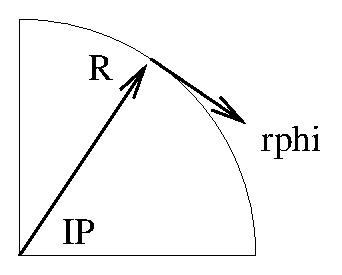
\includegraphics[height=1.7 cm]{global_coordinates}
  \end{minipage} \\
  \begin{minipage}{\linewidth}
    \vspace{0.25 cm}
    local rotations:

    \begin{center}
      \begin{tabular}{c c c}
	$\phi_x$ & $\phi_y$ & \textcolor{red}{$\phi_z$} \\\hline
	70 mrad & 50 mrad & \textcolor{red}{10 mrad}
      \end{tabular}
    \end{center}
  \end{minipage} &
  \begin{minipage}{\linewidth}
    \begin{center}
      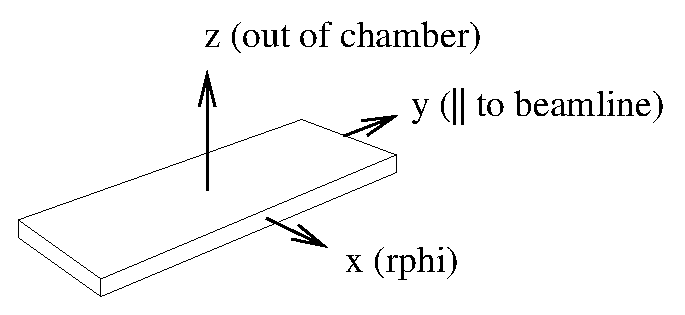
\includegraphics[height=2 cm]{coordinates}
    \end{center}
  \end{minipage} \\
\end{tabular}
\end{frame}

\begin{frame}
\frametitle{How much data do we need?}

$\left.
\mbox{\begin{minipage}{0.8\linewidth}
\vspace{-\baselineskip}
\begin{eqnarray*}
  rphi &\to& \mbox{8 mm $x$-residual} \\
  \phi_z \times L_y &\to& \mbox{25 mm $x$-residual at chamber edge} \\
  \mbox{global } z &\to& \mbox{8 mm $y$-residual} \\
  \phi_z \times L_x &\to& \mbox{20 mm $y$-residual at chamber edge}
\end{eqnarray*}
\end{minipage}}
\right\} \textcolor{red}{\mbox{15-20 mm}}$

\vspace{0.35 cm}
\textcolor{red}{for all barrel chambers} (independent of chamber lengths)

\vfill
Intrinsic resolutions of $\displaystyle \frac{\mbox{endcap}}{\mbox{barrel}} = \frac{\mbox{50 $\mu$m}}{\mbox{170 $\mu$m}}$
\hfill \begin{minipage}{3 cm}
\small (E.\ Torassa, {\it Review of the CMS Muon Detector System})
\end{minipage}

\vfill
\textcolor{red}{5-6 mm for all endcap chambers}

\end{frame}

\begin{frame}
\frametitle{How much data do we need?}

Toy MC was for innermost muon chamber: what about resolution loss in
outer chambers?  Full simulation:

\begin{center}
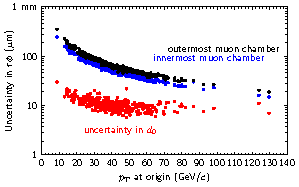
\includegraphics[width=0.7\linewidth]{degradation_of_residuals3}
\end{center}

\vspace{-0.3 cm}
Multiple scattering, non-uniform $\vec{B}$, propagated from tracker
$\Rightarrow$ 30\% widening of distribution
\end{frame}

\begin{frame}
\frametitle{How much data do we need?}

To get 200-300 $\mu$m in barrel and 100-150 $\mu$m in endcap,

\[ \left(1.3 \, \frac{\mbox{20 mm}}{\mbox{300 $\mu$m}}\right)^2 = \mbox{6800}\,\frac{\mbox{muons}}{\mbox{DT}} \mbox{\hspace{0.6 cm}} \left(1.3 \, \frac{\mbox{6 mm}}{\mbox{150 $\mu$m}}\right)^2 = \mbox{2700}\,\frac{\mbox{muons}}{\mbox{CSC}} \]

$\times$ 5 {\small non-overlapping} $=$ 34,000 barrel \mbox{\hspace{0.5 cm}} $\times$ 8 CSCs $=$ 22,000 endcap

\vspace{-0.05 cm}
\hspace{4.5 cm} muons \hspace{3.8 cm} muons

%%         no-cut cross-sec                                              cross-sec * acceptance
%%          0.9 TeV   14 TeV     Br->mu    into detector        0.9 TeV   14 TeV
%% Z        3 nb         60 nb      3.4%             60%               0.06 nb    1.2 nb
%% W      10 nb       180 nb      10%              60%                0.6 nb     11 nb

\begin{center}
\begin{tabular}{l c c c c}
& 0.9 TeV & at \textcolor{gray}{2$\times 10^{33}$} & 1.4 TeV & at \textcolor{gray}{5$\times 10^{34}$} \\ \hline
$Z \to \mu\mu$ in barrel & \textcolor{gray}{1 nb} & \textcolor{gray}{3 years} & \textcolor{gray}{10 nb} & \textcolor{gray}{3 weeks} \\
$Z \to \mu\mu$ in endcap & \textcolor{gray}{1 nb} & \textcolor{gray}{3 years} & \textcolor{gray}{10 nb} & \textcolor{gray}{3 weeks} \\
$W \to \mu\nu$ in barrel & \textcolor{gray}{1 nb} & \textcolor{gray}{3 years} & \textcolor{gray}{10 nb} & \textcolor{gray}{3 weeks} \\
$W \to \mu\nu$ in endcap & \textcolor{gray}{1 nb} & \textcolor{gray}{3 years} & \textcolor{gray}{10 nb} & \textcolor{gray}{3 weeks} \\ \hline
combined & & \textcolor{gray}{all year} & & \textcolor{gray}{one week}
\end{tabular}
\end{center}
\end{frame}

\begin{frame}
\frametitle{Schedule through next year}

\renewcommand{\arraystretch}{1.25}
\begin{tabular}{p{0.18\linewidth} p{0.75\linewidth}}
Deadline & Task \\ \hline

1 Jan, \hfill 2007 & Finish integrating muon chambers into alignment framework \\

1 Mar, \hfill 2008 & Finish development of official HIP alignment \mbox{module} (HIP
is iterative residual minimization) \\

1 Apr & Prototype and study realistic alignment procedure, assuming a
source of muons (full calculation of \#tracks needed) \\
 
1 May & Evaluate possible sources ($W\to\mu\nu$, $Z\to\mu\mu$,
cosmics) and finalize routine (full calculation of \mbox{integrated}
luminosity needed) \\

1 Jun & Document everything
\end{tabular}
\end{frame}

\begin{frame}
\frametitle{Software structure and current status}

CommonAlignment: 3 alignment algorithms share infrastructure

Designed with tracker and muon chambers in mind, but only implemented
for tracker

\begin{itemize}
\item Can move muon chambers (works in local area)
\item Need to calculate muon hit residuals (tools are available)
\end{itemize}

\begin{center}
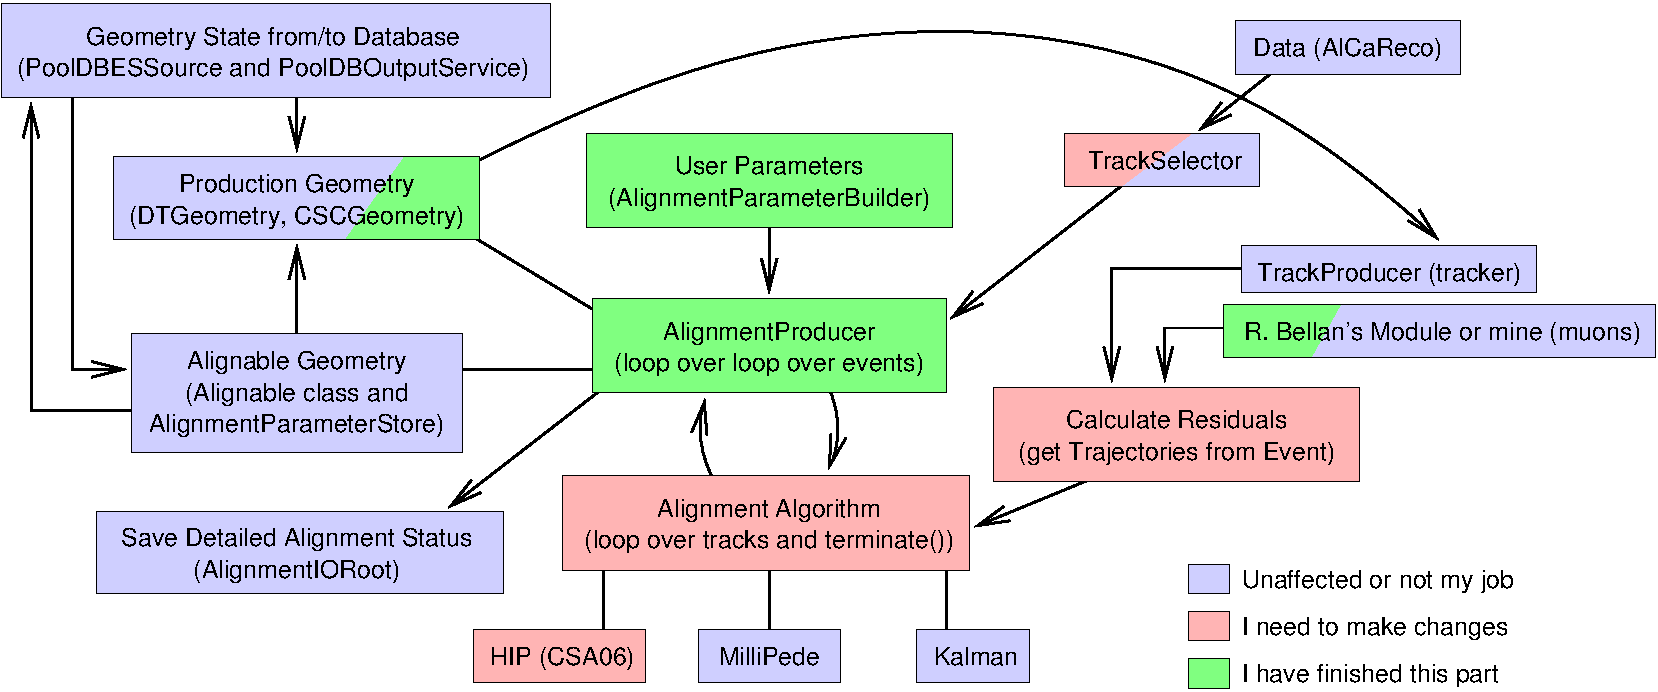
\includegraphics[width=\linewidth]{flow_chart}
\end{center}
\end{frame}

\begin{frame}
\frametitle{Summary}

\begin{itemize}\setlength{\itemsep}{0.25 cm}
\item Track-based and hardware alignment are complimentary because of different systematics

\item But main difference is that hardware alignment is sensitive to
movements on timescales less than \textcolor{gray}{one year (one
week)} for early LHC (normal operation)

\item Can use hardware alignment to find edges of datasets to combine
in track-based alignment

\item Conservative schedule has track-based alignment ready on time

\item Software development is progressing smoothly (well-designed
infrastructure)
\end{itemize}

\label{numpages}
\end{frame}
\end{document}
